\chapter{แบบฝึกหัดการใช้ตารางและสมการ}
จงใช้โครงร่างของแฟ้มต้นฉบับต่อไปนี้ เติมข้อความระหว่าง \lstinline|\begin{document}| กับ \lstinline|\end{document}| เพื่อสร้างเอกสารผลลัพธ์ดังแสดงในหน้าถัดไป

\begin{lstlisting}
\documentclass[10pt]{article}

\usepackage{fontspec}
\usepackage{amsmath}

\setmainfont[Scale=1.2]{TH SarabunPSK}
\XeTeXlinebreaklocale “th_TH”
\setmonofont{LMMono10}

\begin{document}

\end{document}
\end{lstlisting}

สิ่งที่ต้องค้นคว้าเพิ่มเติม
\begin{itemize}
	\item การขีดเส้นบางส่วนของตาราง
\end{itemize}

\newpage
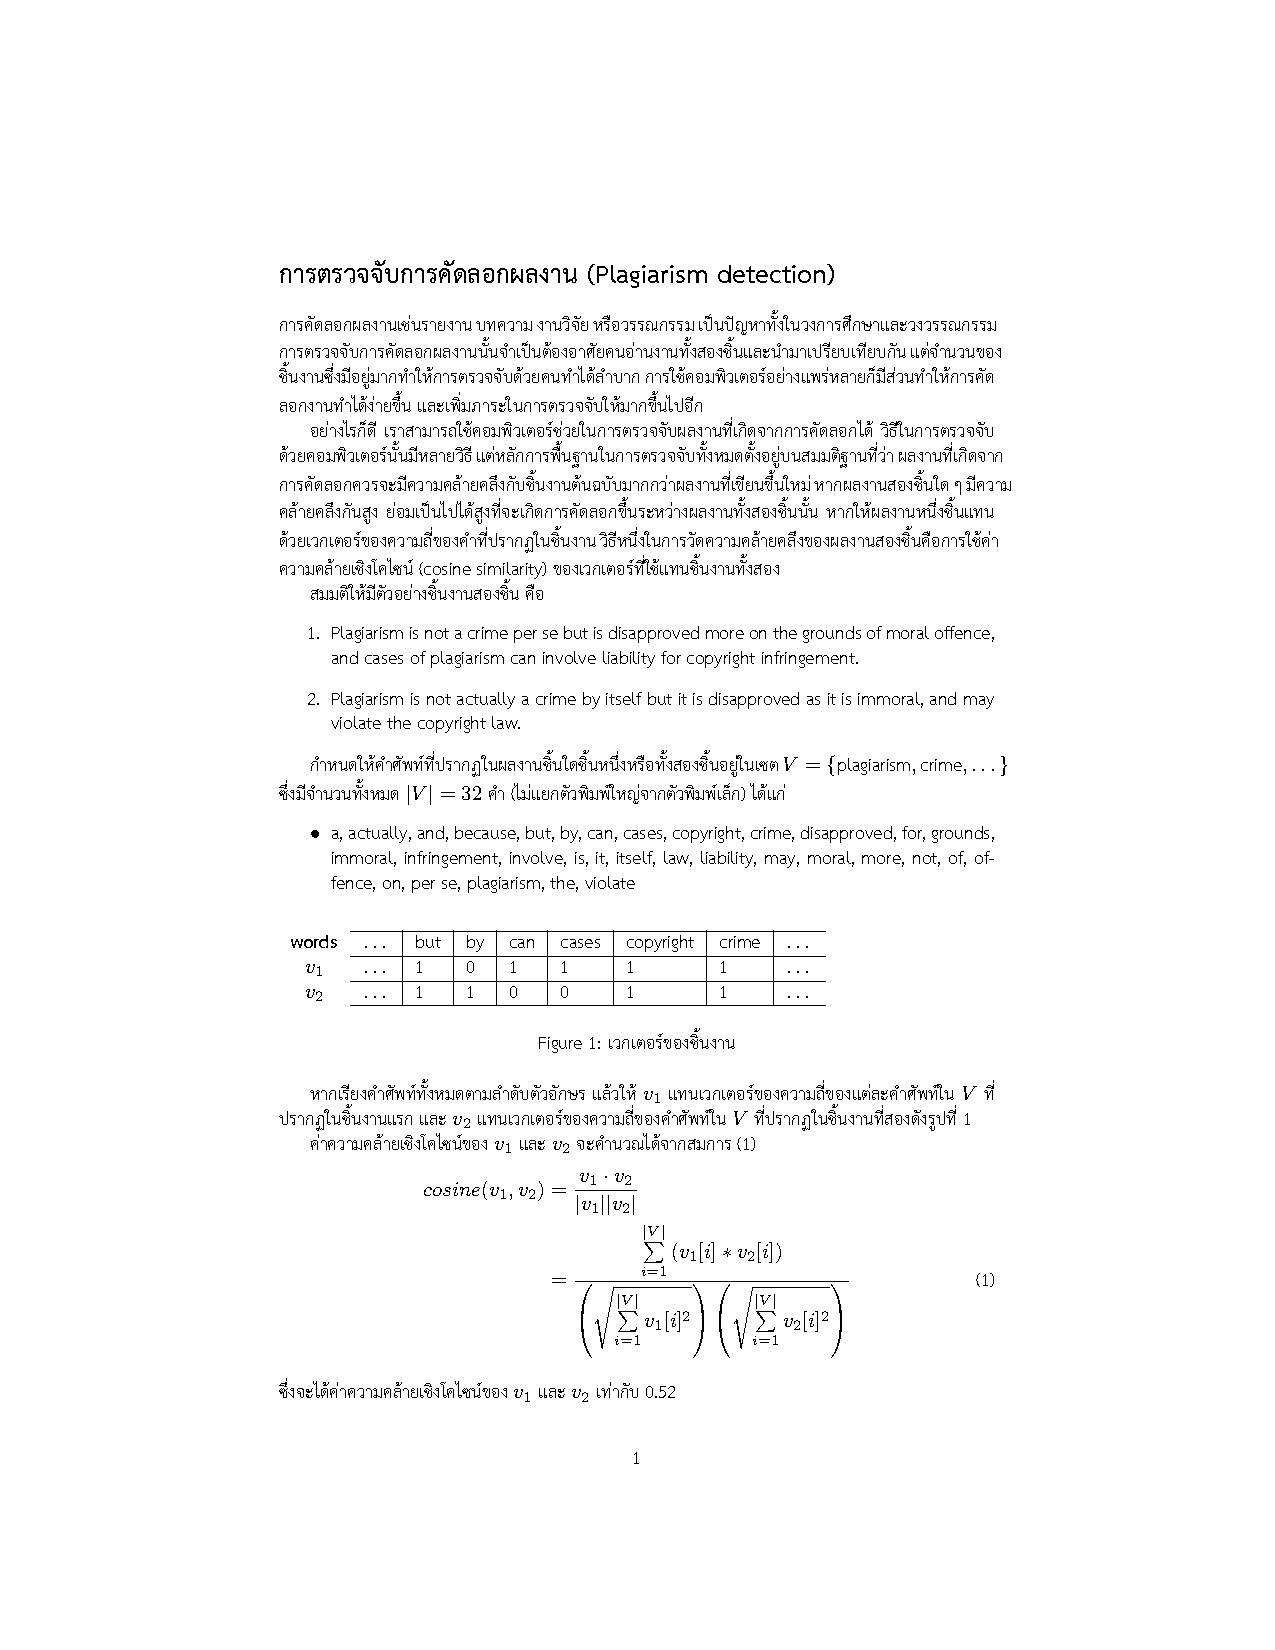
\includepdf{ex2.pdf}
